\documentclass{article}

\usepackage[utf8]{inputenc}
\usepackage[T1]{fontenc}
\usepackage[frenchb]{babel}
\usepackage[top=2cm, bottom=2cm, left=3cm, right=3cm]{geometry}
\usepackage{hyperref}
\usepackage{graphicx}
\usepackage{fancyhdr}
\usepackage{fancybox}

\hypersetup{colorlinks=true}

\title{Snakekans\\-- Projet ISN --}
\author{Luc Chabassier <\href{mailto:luc.linux@mailoo.org}{\nolinkurl{luc.linux@mailoo.org}}> \and Pablo Donato <\href{mailto:pablo.donato@mailoo.org}{\nolinkurl{pablo.donato@mailoo.org}}>}

\begin{document}
\maketitle

\tableofcontents

\section{Introduction.}
Ce programme a été conçu dans le cadre d'un projet d'ISN en 2013. L'objectif était de créer un snake à plusieurs joueurs, permettent à certains serpents d'en coincer.

Le jeu permet jusqu'à quatre joueurs de faire un snake sur une grille constituée de case de 20 pixels sur 20 pixels. Chaque joueur contrôle son serpent à l'aide du clavier (seule les touches fléchées sont utilisable) ou d'une manette (les joysticks et croix directionnelles sont utilisables).

\section{Règles du jeu.}
Le terrain est constitué de cases qui peuvent être vide, contenir un bonus ou contenir un serpent. Chaque joueur peut déplacer son serpent dans les quatre directions, mais il ne peut pas stopper son serpent. Quant un serpent mange un bonus, différentes modifications lui sont appliquées (voir~\ref{bonus}). Il va notamment gagner ou perdre des points et sa taille va varier.

Un serpent meurt quand il heurte un serpent, que ce soit lui-même ou un autre. Lors de sa mort, un malus est appliqué à ses points : si il y a trois serpents vivant lors de sa mort (lui compris), son score est divisé par trois. Si deux serpents meurent en même temps, ils subiront le même malus. La mort est donc extrêmement punitive et un serpent peux donc essayer d'enfermer les autres serpents dans sa queue afin de les faire mourir, imitant un peux le gameplay de jeux comme \emph{armagetron}.

Le jeux se termine lorsqu'il n'y a plus qu'un seul serpent vivant s'il y en avait plusieurs au début ou lors de la mort du seul serpent joueur.

\subsection{Les bonus.} \label{bonus}
% TODO ajouter les images.
Le jeux compte 5 bonus par défaut :\begin{description}
	\item[base] 
\includegraphics{img/base.png} ce bonus à plus grosse fréquence d'apparition. Il rapporte 5 points et augmente la longueur du serpent de 3 cases. Il disparait au bout de 10 secondes.
	\item[big]  
\includegraphics{img/big.png}ce bonus est assez rare, mais surtout il ne reste affiché que 1.5 seconde, ce qui le rend très difficile à attraper. Il rapporte 50 points et augmente la longueur du serpent de 5.
	\item[pic]  
\includegraphics{img/pic.png}ce \emph{bonus} est en fait un malus : il fait perdre 25 points et réduit la taille de 2 cases. Il a une fréquence d'apparition presque aussi élevée que le \emph{base} mais ne reste affiché que 1.5 seconde.
	\item[snake]  
\includegraphics{img/snake.png}ce bonus a une fréquence d'apparition plus faible. Il augmente beaucoup la longueur du serpent; c'est à dire de 10, mais ne rapporte que 2 points. Il disparait au bout de 2 secondes.
	\item[cut]  
\includegraphics{img/cut.png}ce bonus ne rapporte pas de points, mais il réduit la taille du serpent de 5. Il a la même fréquence d'apparition que le bonus \emph{snake}. Il reste par contre affiché 10 secondes.
\end{description}

Chaque bonus est décrit dans un fichier placé dans un dossier spécifique, dont le contenu est scanné à chaque lancement de jeu. Il est donc très simple de modifier, ajouter ou supprimer des bonus.

\subsection{Le serpent.} \label{snake}
Il existe quatre serpents, chacun associé à un joueur. Chaque serpent a une apparence et une couleur différente. Le rouge est la couleur du premier joueur, le vert le second joueur, le bleu le troisième et le jaune le quatrième.

Chaque serpent est chargé depuis une seule image sous la forme d'un tileset. Il suffit donc de changer ces images pour modifier les apparences des serpents pour personnaliser un peu le jeu.

\section{L'interface.}
Les images des interfaces sont susceptibles de changer d'ici à la présentation, mais les changements devraient être mineurs.

\subsection{Le menu.} \label{menu}
\begin{center}
	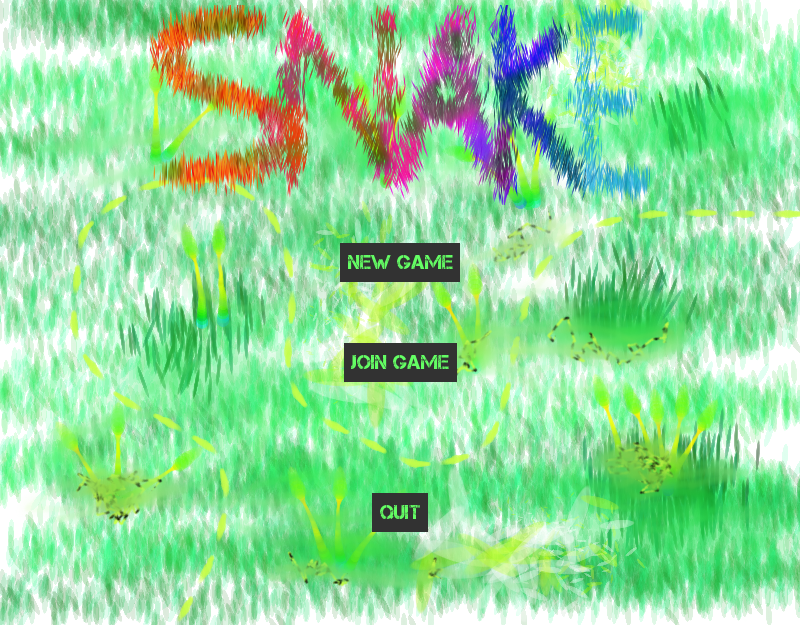
\includegraphics[scale=0.4]{img/menu.png}
\end{center}
Le menu possède trois boutons, en dessous du titre :
\begin{description}
	\item[New Game] Ce bouton permet de lancer une partie. Il amène à l'écran décrit en~\ref{select}.
	\item[Quit] Ce bouton termine le jeu. Il a le même effet que fermer la fenêtre.
\end{description}

L'image du fond est la même dans chaque menu et dans le jeu. C'est une image de taille 800*625 qu'il est facile de changer. Le titre est aussi une image qui peut être changée dans le dossier des ressources.

\subsection{La sélection des joueurs.} \label{select}
\begin{center}
	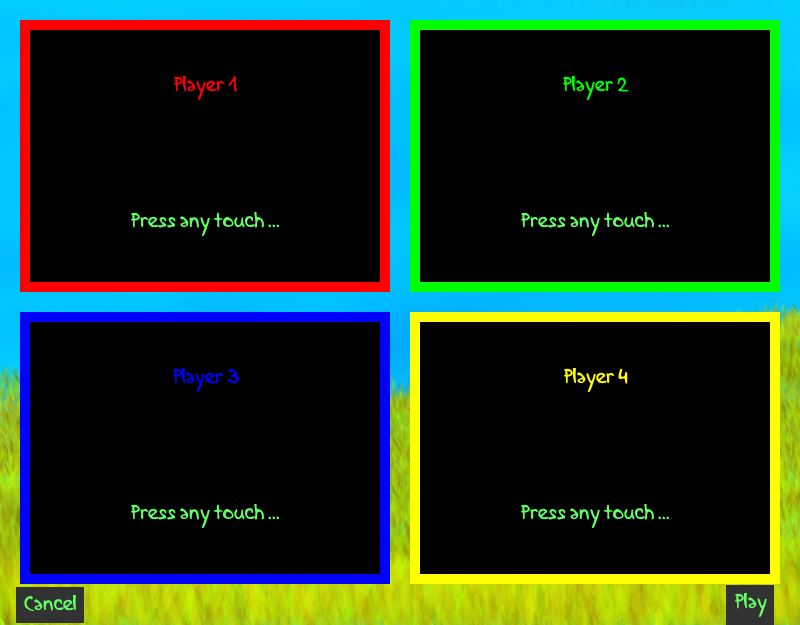
\includegraphics[scale=0.4]{img/empty.png}
\end{center}
Ce menu possède quatre cases. Chaque case correspond à un joueur. Pour ajouter un joueur, il faut laisser appuyé un bouton sur le controleur (joystick ou clavier) qu'il souhaite utiliser jusqu'à ce qu'une jauge ait finit de se remplir. Les conexions de clients apparaissent aussi ici. Cette interface est inspirée de celle du jeu indépendant \emph{Jamestown}.

Ce menu avec un clavier et un joystick connecté ressemble à :
\begin{center}
	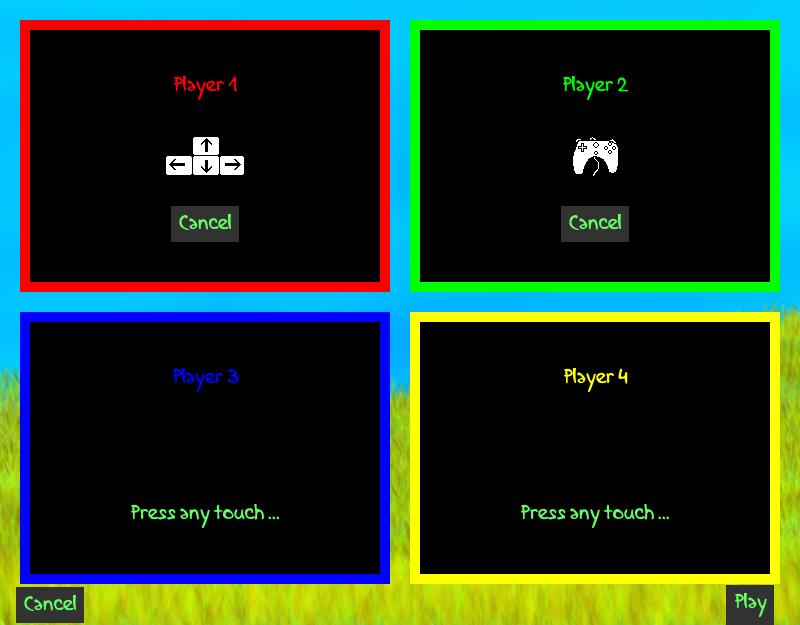
\includegraphics[scale=0.4]{img/full.png}
\end{center}

Ce menu possède deux boutons :
\begin{description}
	\item[Cancel] Ce bouton ramène au menu général, décrit en~\ref{menu}.
	\item[Play] Ce bouton lance un jeu (voir~\ref{game}) avec les joueurs connectés.
\end{description}

\subsection{Le jeu.} \label{game}
\begin{center}
	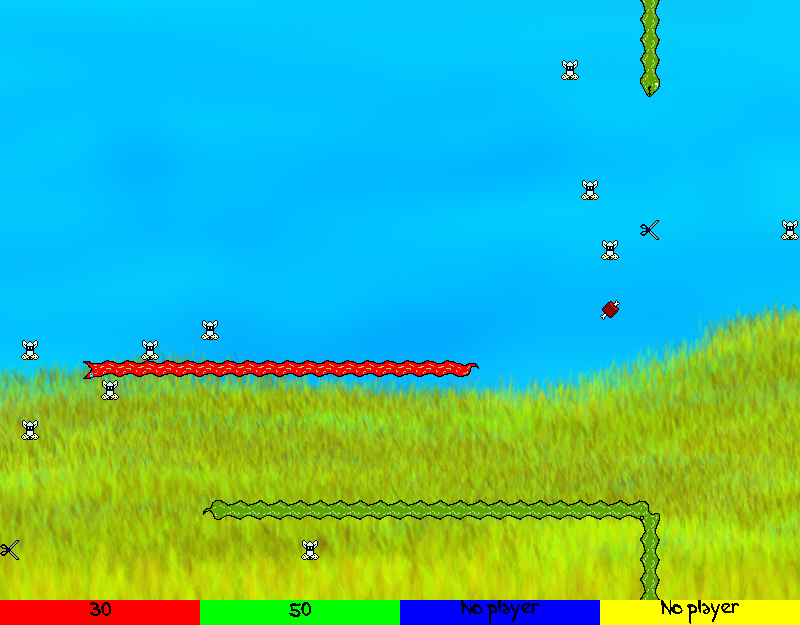
\includegraphics[scale=0.4]{img/game.png}
\end{center}
On remarque sur cette capture d'écran deux serpents, donc deux joueurs connectés, ainsi que divers bonus. En bas de l'écran se trouve la barre qui indique le score des joueurs.

Lorsque le jeu est terminé, il se stoppe pendant deux secondes, permettant de comprendre ce qui a causé la mort du dernier serpent, puis on arrive sur cet écran :
\begin{center}
	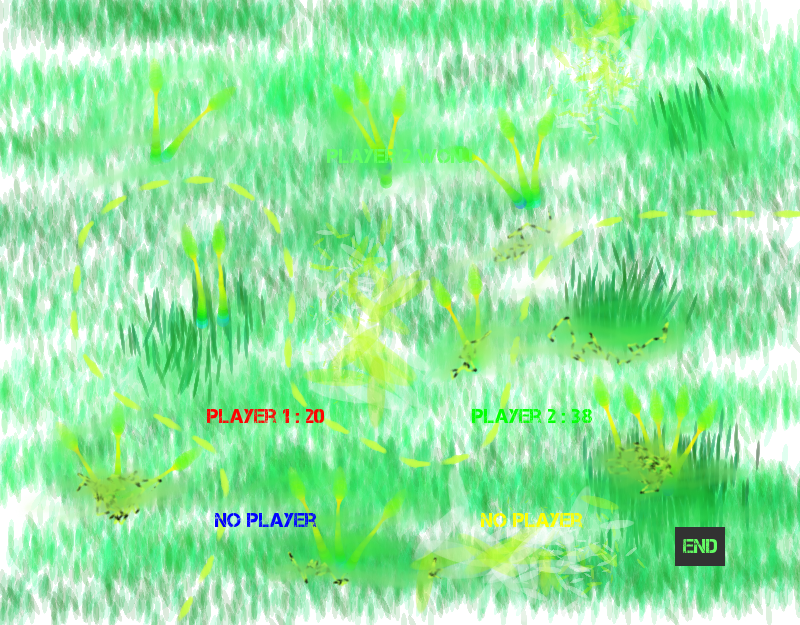
\includegraphics[scale=0.4]{img/game_over.png}
\end{center}
Cet écran affiche le score de chaque joueur par ordre décroissant ainsi que le gagnant. Le bouton \emph{End} permet de retourner à l'écran de sélection des joueurs (partie~\ref{select}) avec les joueurs connectés comme avant la partie, permettant de relancer une partie très rapidement.

\section{Développement.}
\subsection{Bibliothèques utilisées.}
Ce jeu est codé en c++, en utilisant la dernière norme \emph{c++11}, et utilise certaines bibliothèques SDL : tout d'abord la bibliothèque \href{http://www.libsdl.org/}{SDL} de base, avec ses extensions \href{http://www.libsdl.org/projects/SDL\_image/}{SDL\_image}, \href{http://www.libsdl.org/projects/SDL\_ttf/}{SDL\_ttf} et \href{http://www.libsdl.org/projects/SDL\_mixer/}{SDL\_mixer}. Certaines bibliothèque \href{http://www.boost.org/}{boost} sont elles aussi utilisées : \href{http://www.boost.org/doc/libs/1\_39\_0/libs/filesystem/doc/index.htm}{boost.filesystem} et \href{http://www.boost.org/doc/libs/1\_53\_0/libs/regex/doc/html/index.html}{boost.regex}.

Ce cahier des charges est rédigé en \href{http://www.latex-project.org/}{\LaTeX}.

\subsection{Outils.}
L'outil utilisé pour écrire le code est \href{http://www.vim.org/}{Vim} (éditeur et colorateur). Le code est versionné avec \href{http://git-scm.com/}{git} (le code est hébergé sur \href{https://github.com/Lycee/ISN\_snake}{github}) et la chaine de compilation est générée par \href{http://www.cmake.org/}{Cmake}. Le jeu est dévellopé sous \href{https://en.wikipedia.org/wiki/Linux}{GNU/Linux} mais devra être compatible avec d'autre plateforme comme Windows ou Mac.

\subsection{Correction des bugs.}
Le code a subit des tests de couverture de code à l'aide de \href{http://gcc.gnu.org/onlinedocs/gcc-4.5.2/gcc/Gcov.html#Gcov}{gcov}.

La détection des sources des bugs a été faite à l'aide de \href{https://www.gnu.org/software/gdb/}{gdb} et la détection des fuites de mémoire a été permise par \href{http://www.valgrind.org/}{valgrind}.

\section{Licence.}
Le code est sous licence \href{http://gplv3.fsf.org/}{GNU GPLv3} (voir le fichier LICENCE fournit avec le code), au copyright de Luc Chabassier et Pablo Donato.

Les ressources graphiques (images, tileset) ont été crées par Luc Chabassier à l'aide de \href{http://www.gimp.org/}{Gimp} et de \href{http://mypaint.intilinux.com/}{MyPaint}, et sont sous licence \href{https://creativecommons.org/licenses/by-sa/2.0/}{CC-BY-SA}. Remerciement particuliers à Lucas Saliou, pour ses conseils pour l'esthétique du jeu.

Les sons et musiques sont tirées du jeu \href{http://supertux.lethargik.org/}{SuperTux2}, et sont sous licence \href{https://creativecommons.org/licenses/by-sa/2.0/}{CC-BY-SA}.

La police d'écritue utilisée est la \href{http://openfontlibrary.org/en/font/lenka-stabilo}{Lenka Stabilo}, obéissant à la licence libre \href{http://www-old.gnome.org/fonts/}{Bitstream Vera License}.

Ce document lui-même et ses sources sont sous licence \href{https://creativecommons.org/licenses/by-sa/2.0/}{CC-BY-SA}.

\end{document}

